\documentclass[12pt]{ctexart}
\usepackage{amsmath,graphicx,textcomp,subfigure,indentfirst,ctex,color,float}
\usepackage{bm, mhchem}
\title{Lecture 12}
\date{\today}
\newcommand{\new}[1]{\textcolor{blue}{#1}}

\newcommand{\refeq}[1]{式~(\ref{#1})}
\newcommand{\refeqs}[2]{式~(\ref{#1}) - (\ref{#2})}
\newcommand{\reffig}[1]{图~(\ref{#1})}
\begin{document}

\maketitle

% \section{线性微扰理论(续)}

% 对于超视界的涨落 (Super-Horizon perturbation), 即 $\lambda > \lambda_{\rm{H}}$,
% 有 $\Phi_{\vec{k}}=\rm{const.}$
% 所以 
% \begin{equation}
%     -k^{2} \Phi_{\vec{k}}=4 \pi G a^{2} \bar{\rho} \delta_{\vec{k}} \quad \Rightarrow \quad \delta_{\vec{k}} \propto\left(\bar{\rho} a^{2}\right)^{-1}
% \end{equation}
% $\delta_{\vec{k}}$ 随着 $\left(\bar{\rho} a^{2}\right)^{-1}$ 增长。

% 对于视界以内的涨落 (Sub-Horizon perturbation), 即 $\lambda < \lambda_{\rm{H}}$, 在辐射主导时期,这些涨落会震荡。

% %%%%%%%%%%%%%%%%%%%%%%%%%%%%%%%%%%%%%%%%%%%%

% % 其实 $\delta \propto  \delta_{+}$, 也不需要物质主导。
% % $$
% % g(z) \approx \frac{5}{2} \Omega_{m}(z)\left\{\Omega_{m}^{4 / 7}(z)-\Omega_{\Lambda}(z)+\left[1+\frac{\Omega_{m}(z)}{2}\right]\left[1+\frac{\Omega_{\Lambda}(z)}{70}\right]\right\}^{-1}
% % $$
% % matter dominated era
% 在物质主导期($\Omega_M\approx 1$),
% \begin{equation}
%     \delta_{+}  \propto  t^{2/3} \propto a =\frac{1}{1+z}
% \end{equation}

% 将 $\delta_{\vec{k}}$   的空间部分和时间部分分开: $\delta_{\vec{k}}(t) = \delta_{\vec{k}}(t_0) D(t)$, 其中 定义了 $D(t)$ 是线性增长率(linear growth rate), 写做 红移的函数为 $D(z)=g(z)/(1+z)$.
% 此时 
% \begin{equation}
%     \delta_{+} \propto D(t) \propto a =\frac{1}{1+z}
% \end{equation}

% % ----
% % Silk damping 会擦除全部的消除的 重子涨落 ,到recombination。 

% % ----

% \reffig{fig:Bary_pert} 总结了考虑宇宙膨胀时的重子涨落情况。

% 因为 Silk damping 的存在,到recombination时,所有小尺度的 重子涨落都被擦除,
% 结构形成只能是大尺度的涨落先涨起来,然后再逐渐过渡到小尺度,这叫做
% Top-down Scenario.
% 但 Top-down Scenario
% 存在一些问题:
% 在 Top-down Scenario 中,要形成今天的大尺度结构,需要 recombination 时
% 的物质涨落 $|\delta_m|> 10^{-3}$. 
% 而物质涨落和CMB涨落相联系
% $\frac{\delta T}{T}=\frac{1}{4} |\delta_r| = \frac{1}{4} \times \frac{4}{3} |\delta_m| \sim 10^{-3}$.
% 早期CMB的测量就排除了 Top-down Scenario. 今天测量到 CMB涨落约为 
% $\frac{\delta T}{T} \sim 10^{-5}$.

% 可见仅有重子涨落 无法解释现有的观测迹象,需要另一种物质来提供涨落,这就是暗物质。
% % Peebles 等 发展了 新的模型: recombination之前 isothermal perturbation,
% % 此时 声速很小,所以金斯尺度也很小, 没有 Silk damping . 金斯mass 1e6 M_sun
% %  bottom-up
% % CMB涨落还是太大
% %  isothermal perturbation un-natural
% % 重子的 perturbation 无法解释现有的观测迹象,需要

% \begin{figure}[!hbtp]
% 	\centering 
% 	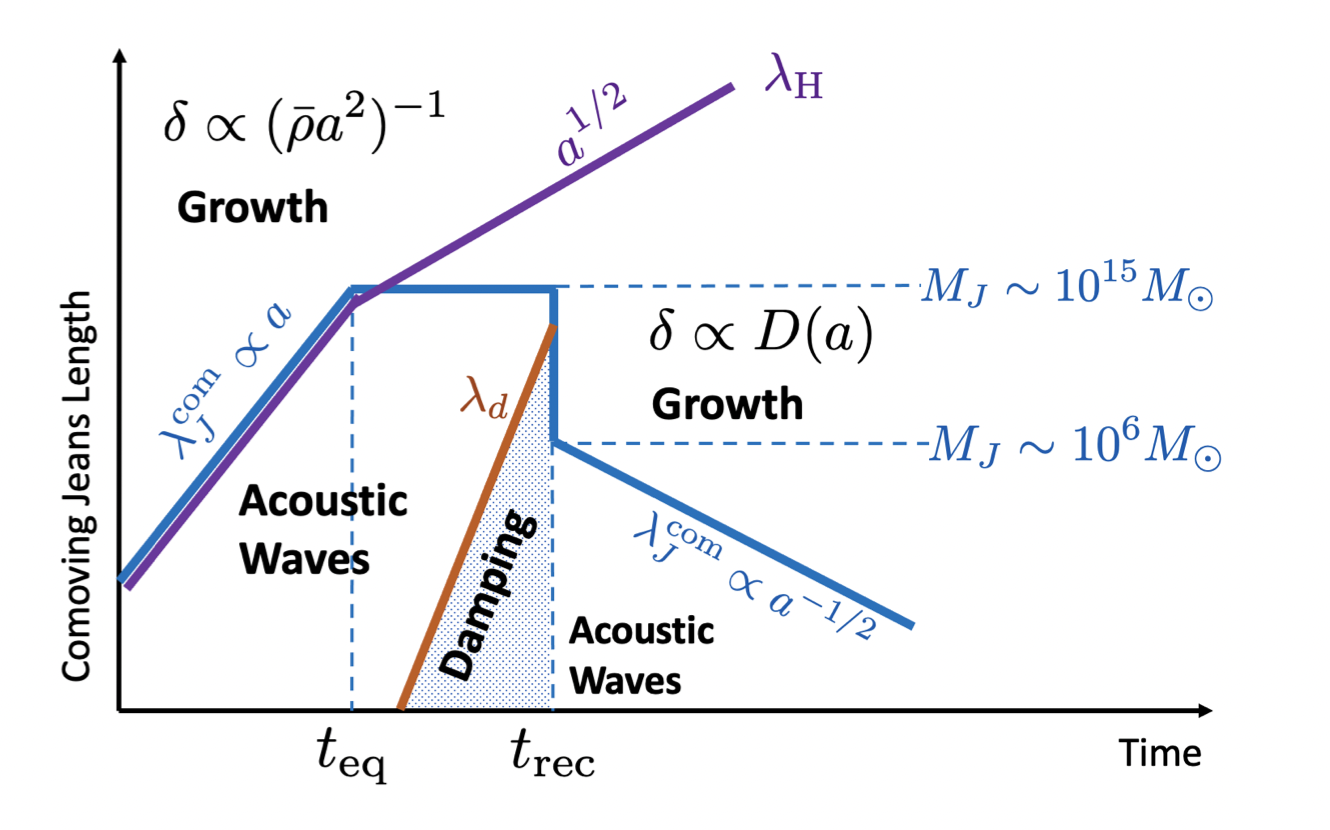
\includegraphics[width=1.0\linewidth]{Baryon_pert_H.png}
% 	\caption{考虑宇宙膨胀时的重子涨落}
%     \label{fig:Bary_pert}
% \end{figure}
% %%%%%%%%%%%%%%%%%%


\section{Dark Matter Perturbation}

暗物质是不与 光子 发生 相互作用的物质,
目前尚不清楚它的本质,可能是某些未被发现的“新粒子”,在宇宙早期脱离热平衡遗留下来 (thermal relics),
也有模型不是热平衡遗留造成的。
目前主要有以下几类暗物质模型:
% 以 在退耦时 是否相对论性 区分
\begin{itemize}
    \item 冷暗物质(cold dark matter, CDM):粒子运动速度较低的暗物质模型。除了不和重子物质作用外,自身相互作用也很小。最有名的如 WIMP 微弱作用大质量粒子 (Weakly Interacting Massive Particals) .
    \item 热暗物质(hot dark matter, HDM):粒子热运动速度较大的暗物质模型。比如退耦后的中微子。
    \item 其它暗物质模型:Non-thermal relics, 不是脱离热平衡而来。比如 轴子 axions, 磁单极子monopoles, 宇宙弦 cosmic strings,其中后两者都属于宇宙的拓扑缺陷(topologecial defects)
\end{itemize}

目前宇宙学观测比较倾向冷暗物质,我们以下也 用冷暗物质模型 考虑暗物质涨落。

冷暗物质是无碰撞粒子,不能使用流体力学方程。

我们用到
连续性方程
\begin{equation}
    \frac{\partial \delta}{\partial t}+\frac{1}{a} \nabla \cdot[(1+\delta) \vec{v}]=0
\end{equation}
和金斯方程(类比流体力学的欧拉方程)
\begin{eqnarray}
    \frac{\partial \vec{v}}{\partial t}+\frac{\dot{a}}{a} \vec{v}+\frac{1}{a}(\vec{v} \cdot \nabla) \vec{v} =-\frac{\nabla \Phi}{a} - \frac{\sigma^2}{a}\frac{\nabla \delta}{1+\delta}
\end{eqnarray}
用 $\sigma$ 替换了欧拉方程中的 $c_s$.
其中定义了 速度色散 (velocity dispersion tensor)
$\sigma_{ij} \equiv\left\langle v_{i} v_{j}\right\rangle-\left\langle v_{i}\right\rangle\left\langle v_{j}\right\rangle$
在各向同性假设下 $\sigma_{ij}=\sigma\delta_{ij}$,
加上均匀性假设 $\sigma=\left\langle v_i^2 \right\rangle ^{1/2}$.

对比流体力学方程可得 金斯尺度 
\begin{equation}
    \lambda_{\mathrm{J}}^{\text {prop }}=a(t) \lambda_{\mathrm{J}}^{\text {com }}=a(t) \frac{2 \pi}{k_{\mathrm{J}}}=\sigma \sqrt{\frac{\pi}{G \bar{\rho}}}
\end{equation}
$\lambda > \lambda_{\rm{J}}$时,涨落在引力作用下增长(gravitational collapse).
$\lambda < \lambda_{\rm{J}}$时,无碰撞的暗物质粒子会将 涨落抹掉,而不是以波的形式存在,叫做 free streaming damping.


在辐射主导时期,
\begin{equation}
    \frac{d^{2} \delta_{\vec{k}} }{d t^{2}}+2 \frac{\dot{a}}{a} \frac{d \delta_{\vec{k}}}{d t}=4 \pi G\left(\bar{\rho}_{m}+\bar{\rho}_{r}\right) \delta_{\vec{k}} \quad \Rightarrow \quad \delta_{+} \propto 1+\frac{3 \bar{\rho}_{m}}{2 \bar{\rho}_{r}}=1+\frac{3 a}{2 a_{\mathrm{eq}}} 
\end{equation}
当 $a\ll a_{\rm{eq}}$, $\delta_{+}\propto 1$,涨落停滞,即使大于金斯尺度也不会增长(Stagnation),也称为 Meszaros 效应。

可见在辐射主导区,各尺度的暗物质涨落都无法增长,需要等到 $t_{\rm{eq}}$ 之后才能增长。

小尺度的结构先形成,继而碰撞形成大尺度的结构,这叫做 Bottom-up Scenario.
暗物质先形成 非线性 结构,重子物质落入 暗物质涨落形成的引力势阱中,
形成恒星与星系。

\reffig{fig:CDM_pert} 总结了暗物质涨落。
\begin{figure}[!hbtp]
	\centering 
	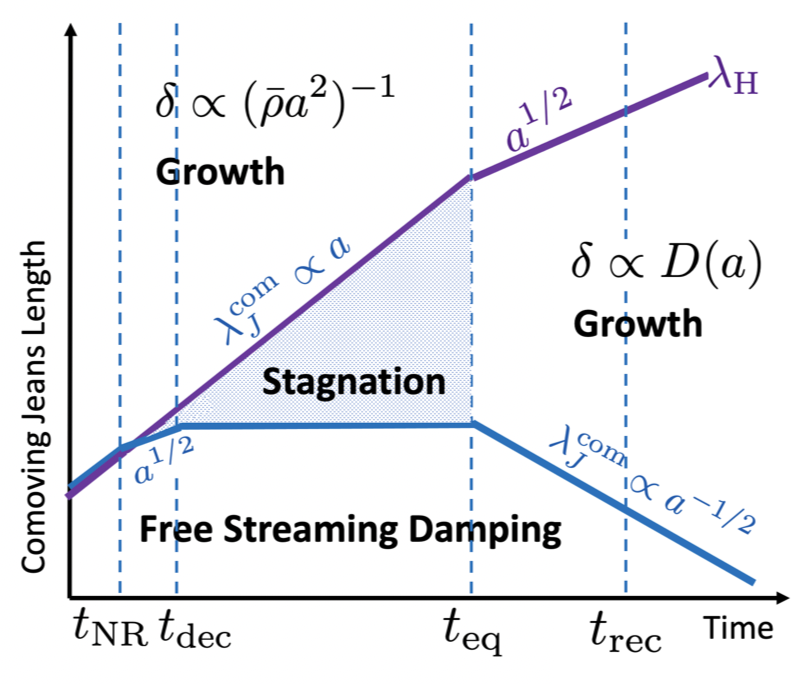
\includegraphics[width=1.0\linewidth]{CDM_pertu.png}
	\caption{冷暗物质模型给出的暗物质涨落}
    \label{fig:CDM_pert}
\end{figure}

\section{非线性结构}
以上都是线性微扰理论,只适用于 $\delta \ll 1$ 的情况,在 recombination ($\delta\sim 10^{-5}$) 前后是适用的。而今天的星系都属于 $\delta \gg 1$ 的非线性结构,在本节中我们考虑非线性结构。

非线性结构 不能用高斯场,  不同模之间不独立,不能用简单的 growth rate 来表示涨落的增长。
% 原则上没有解析解。

处理非线性结构有以下几种方法:
\begin{itemize}
    \item 最“精确”的方法是数值模拟,但是也受到算法的影响。
    \item 在 quasi-linear 区域可以用 高阶的微扰论。
    \item Oversimplified analytical models 不准确,但可以给我们一些物理直觉。
\end{itemize}
我们的课程将介绍部分 Oversimplified analytical models.

\subsection{Spherical Collapse (SC) model}

我们考察均匀宇宙中的一个球状高密度区 $\delta>0$. 简单起见,我们假设宇宙中只有物质,没有暗能量。

把这个球状高密度区分成一层层球壳,
% 只考虑暗物质,所以是 collision-less 的。
% 球壳可以各自 oscillates 而不会互相影响。
不失一般性,考察某个球壳上的一个质点,
假设在某个 初始时刻, 该球形高密度区的半径是 $r_i$, overdensity 是 $\delta_i$, 背景宇宙的平均密度是 $\bar{\rho}_i$.
牛顿万有引力定律告诉我们,只有内层的物质对外层有引力,且等效于内层的全部质量集中于球心。
\begin{eqnarray}
    M=M(r<r_i)=\frac{4}{3} \pi r_{i}^{3} \bar{\rho}_{i}\left[1+\delta_{i}\right]=\frac{4}{3} \pi r^{3}(t) \bar{\rho}(t)[1+\delta(t)]
\end{eqnarray}
质点只受万有引力,根据牛顿定律, $\ddot{r}=-\frac{GM}{r^2}$. 
积分可以得到 比能(specific energy) $E=\frac{1}{2} \dot{r}^{2}-\frac{G M}{r}$. 如果比能大于0,该层球壳可以一直膨胀,如果比能小于0,该层球壳就会在有限时间内坍缩。

如果比能 $E=0$, 
\begin{equation}
    r(t)=(9 G M / 2)^{1 / 3} t^{2 / 3} \propto t^{2 / 3}
\end{equation}
而宇宙膨胀速率 $D(a) = a\propto t^{2 / 3}$,球状区域和宇宙同步膨胀,涨落不增长 $\delta(t) = \delta_i$.

在初始时刻,
% the initial velocity of the mass shell can be simply approxiamted as the Hubble flow.
\begin{equation}
    \begin{aligned}
        E_{i} &=K_{i}+W_{i}=\frac{1}{2} v_{i}^{2}-\frac{G M}{r_{i}}=\frac{1}{2}\left(\dot{a} x_{i}+a \dot{x}_{i}\right)^{2}-\frac{G}{r_{i}}\left[\frac{4}{3} \pi r_{i}^{3} \bar{\rho}_{i}\left(1+\delta_{i}\right)\right] \\
        & \approx \frac{1}{2} H_{i}^{2} r_{i}^{2}-\frac{1}{2} H_{i}^{2} r_{i}^{2}\left(1+\delta_{i}\right)=K_{i}-K_{i}\left(1+\delta_{i}\right)=-K_{i} \delta_{i}
    \end{aligned}
\end{equation}
其中忽略了  $a \dot{x}_{i}$, 且用到了 
$\frac{1}{2} H_{i}^{2} r_{i}^{2} = \frac{G}{r_i} \times \frac{4}{3} \pi r_{i}^{3} \bar{\rho}_{i}$.
% $H^2 = \frac{8}{3} \pi G \bar{\rho}$.
(对平均密度的宇宙,比能$E=0$)

若 $\delta_i>0$, 则 $E_i<0$, 对于只有物质没有暗能量的宇宙来说,高密度区总是会坍缩。

球壳的运动方程可以用以下参数方程组表示
\begin{equation} \label{eq:EoM}
    r=A(1-\cos \theta), \quad 
    t=B(\theta-\sin \theta), \quad
    \theta \in[0,2 \pi]
\end{equation}
\begin{equation}
    A=\frac{G M}{2|E|}, \quad
    B=\frac{G M}{(2|E|)^{3 / 2}}
\end{equation}

$\theta=0$ 时, $t=0$ ,球壳开始膨胀,
在 $\theta=\pi$ 时到达最大半径,开始折回来 (turn around),
当 $\theta= 2\pi$ 前,这团高密度球完成维里化,完成引力坍缩。
\begin{equation}
    t_{\rm{collapse}} = 2 t_{\rm{ta}}
\end{equation}

整个过程中能量守恒。
\begin{eqnarray}
    E_{\rm{ta}}  &=& -\frac{GM}{r_{\rm{max}}} = -\frac{H_i^2 r_i^3}{2 r_{\rm{max}} } (1+\delta_i) \\ 
    E_i &=& -K_i \delta_i = -\frac{1}{2} H_i^2 r_i^2 \delta_i
\end{eqnarray}

\begin{equation} \label{eq:r_max}
    E _{\rm{ta}} = E_i \quad \Rightarrow \quad \frac{r_{\max }}{r_{i}}=\frac{1+\delta_{i}}{\delta_{i}} \approx \delta_{i}^{-1}
\end{equation}
最后一步假设了 $\delta_i \ll 1$.

\refeq{eq:r_max} 说明 球壳膨胀的最大半径只与 初始的 overdensity 有关,与球壳内包含的质量绝对值无关。
% 越小的 perturbation turn around 越晚,膨胀得越大。

根据 \refeq{eq:EoM} 可以推知 overdensity 的演化:

1. 球形区的密度
\begin{equation}
    \rho=\frac{3 M}{4 \pi r^{3}}=\frac{3 M}{4 \pi A^{3}}(1-\cos (\theta))^{-3}
\end{equation}

2. 背景的密度
\begin{equation}
    \bar{\rho}=\frac{1}{6 \pi G t^{2}}=\frac{1}{6 \pi G B^{2}}(\theta-\sin \theta)^{-2}
\end{equation}

3. 所以 球形区的 overdensity是
\begin{equation}
    1+\delta=\frac{\rho}{\bar{\rho}}=\frac{9}{2} \frac{(\theta-\sin \theta)^{2}}{(1-\cos \theta)^{3}}
\end{equation}
初始条件,即 $\theta \ll 1$ 时,利用泰勒展开可以得到
\begin{equation}
    \delta_{i}=\frac{3}{20}(6 \pi)^{2 / 3}\left(\frac{t_{i}}{t_{\rm{ta} }}\right)^{2 / 3}
\end{equation}
% 对于一块均匀的高密度球,各球壳会一起坍缩。

在线性理论中, 我们得到 $\delta_{\text {lin }} \propto D(a) \propto a \propto t^{2 / 3}$, 所以线性扰动随时间变化的关系为
\begin{eqnarray}
    \delta_{\operatorname{lin}}(t)=\delta_{i}\left(\frac{t}{t_{i}}\right)^{2 / 3}=\frac{3}{20}(6 \pi)^{2 / 3}\left(\frac{t}{t_{\rm{ta} }}\right)^{2 / 3}
\end{eqnarray}

比较两种理论给出的 overdensity:

在 turn-around 时刻,
% SC model: $1+\delta=\frac{9}{2} \frac{(\theta-\sin \theta)^{2}}{(1-\cos \theta)^{3}}$
% - Linear theory: $\delta_{\operatorname{lin}}=\frac{3}{20}(6 \pi)^{2 / 3}\left(\frac{t}{t_{\max }}\right)^{2 / 3}$
% t turn-around =t_{\text {,ax }}
$\left(t_{\mathrm{ta}} , \theta=\pi\right)$ :
\begin{itemize}
    \item $\mathrm{SC}$ model: $1+\delta\left(t_{\mathrm{ta}}\right)=\frac{9 \pi^{2}}{16} \approx 5.55$
    \item Linear theory: $\delta_{\text {lin }}\left(t_{\mathrm{ta}}\right)=\frac{3}{20}(6 \pi)^{2 / 3} \approx 1.062$
\end{itemize}


在 collapse 时刻,
% (shell crossing) 
$\left(t_{\text {coll }}=2 t_{\mathrm{ta}}  , \theta=2\pi\right)$ :
\begin{itemize}
    \item SC model: $\delta\left(t_{\text {coll }}\right)=\infty$
    \item Linear theory: $\delta\left(t_{\text {coll }}\right)=\frac{3}{20}(12 \pi)^{2 / 3} \approx 1.686$
\end{itemize}



定义 critical overdensity for collapse $\delta_c = 1.686$, 在考虑暗能量存在的情况下, $\delta_c$ 只有约 1\% 的修正,一般使用近似值 1.686.
% for collapse regions 
当 $\delta_{\rm{lin}} > \delta_c$ ,该区域就会坍缩。
最后会维里化,形成 virialized dark matter halo.
% 这个球的随时间的演化 见 



维里化后, 
\begin{equation}
    2K_f + W_f = 0
\end{equation}
其中 $f$代表final,最终状态。

总能量 $E_f = K_f + W_f = \frac{1}{2} W_f = -\frac{GM}{2 r _{\rm{vir}} }$.
而 turn-around 时,全部能量来自势能 $E _{\rm{ta}} = W _{\rm{ta}} =-\frac{GM}{r _{\rm{ta}} }$,
由能量守恒 得到 $r _{\rm{vir}} =\frac{1}{2} r _{\rm{ta}} $,
进而
$\rho _{\rm{vir}} = 8 \rho _{\rm{ta}} $. 
% \new{而 $\rho _{\rm{ta}} $ 可以用 SC model 计算得到,这样我们就能解析地得到维里化后的密度。}

利用 $\bar{\rho} \propto a^{-3} \propto t^{-2}$ 和
$t _{\rm{coll}} = 2 t _{\rm{ta}} $
得到
维里化的暗物质晕的平均 overdensity 是
\begin{eqnarray}
        1+\Delta_{\mathrm{vir}} &\equiv& 1+\delta\left(t_{\text {coll }}\right)=\frac{\rho\left(t_{\text {coll }}\right)}{\bar{\rho}\left(t_{\text {coll }}\right)}=  \frac{8 \rho\left(t_{\mathrm{ta}}\right)}{\bar{\rho}\left(t_{\mathrm{ta}}\right) / 4} \\ 
        &=& 32\left[1+\delta\left(t_{\mathrm{ta}}\right)\right]=32 \times \frac{9 \pi^{2}}{16} = 18\pi^2 \approx 178
\end{eqnarray}

人们经常用这个判据来在 N-body simulation 中认证 dark matter halos.

线性微扰理论, SC model 以及维里化 对暗物质晕形成的 描述 总结在 \reffig{fig:SC_model} 中。
\begin{figure}[!hbtp]
	\centering 
	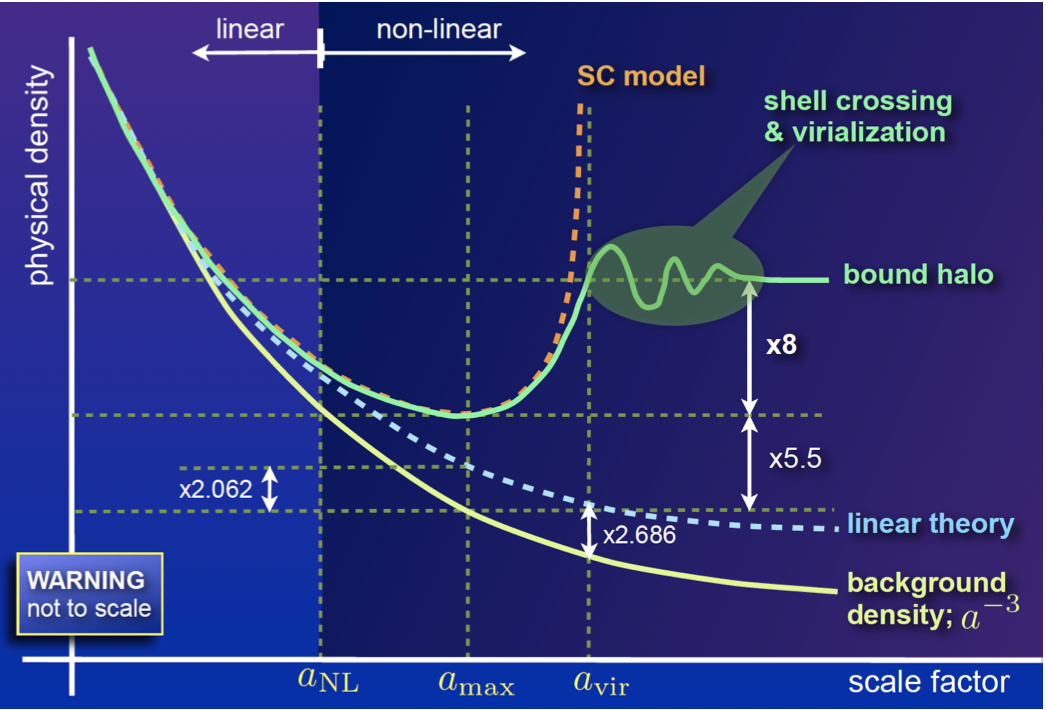
\includegraphics[width=1.0\linewidth]{SC_model.png}
	\caption{halo的形成}
    \label{fig:SC_model}
\end{figure}



\subsection{椭球坍缩}
实际情况中往往是椭球坍缩而非完全对称的球坍缩。

椭球高密度区的坍缩(Ellipsoidal Collapse)
与球形高密度区的区别在于三个旋转轴不对称。
最短轴的方向会先坍缩,由椭球变成饼(sheet / pancake / Zel'dovich pancake),可以用 Zel'dovich 近似 解释。
然后会沿着第二短轴坍缩,变成线型 (filament),
最后剩下的一个轴坍缩,形成球状的暗物质晕 (halo)。 
如 \reffig{fig:Ellips_Colla} 所示。

\begin{figure}[!hbtp]
	\centering 
	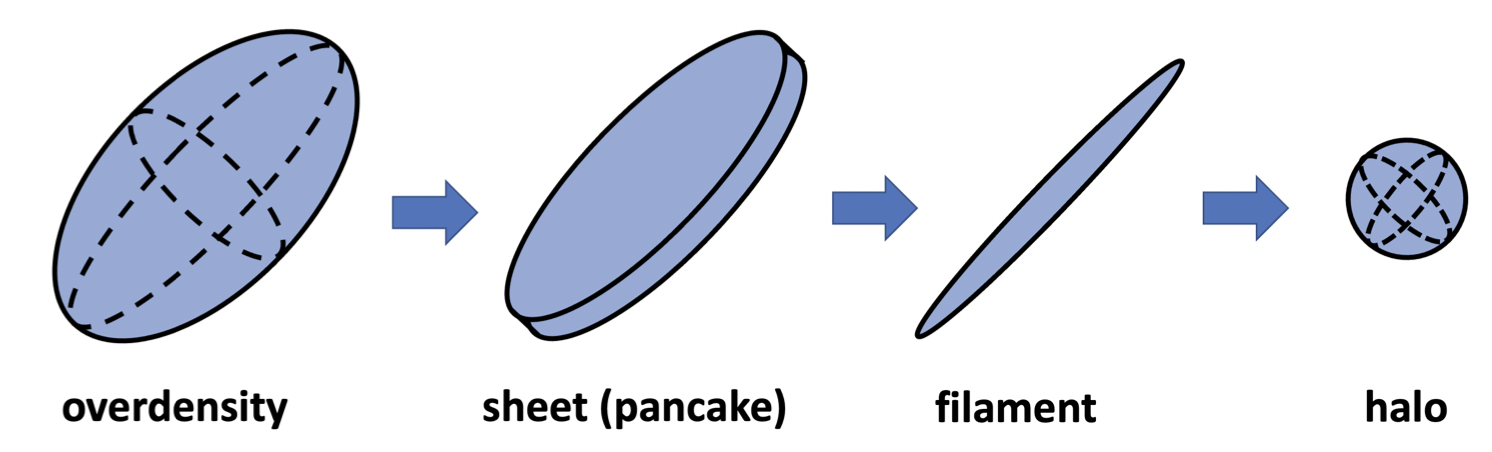
\includegraphics[width=1.0\linewidth]{Ellips_Colla.png}
	\caption{椭球坍缩示意图}
    \label{fig:Ellips_Colla}
\end{figure}

\section{暗物质晕的结构}

暗物质晕内部的密度并不是均匀的。我们可以用一些解析的模型来描述。

\subsection{power-law density profile}

最简单的是 幂律谱模型 (power-law density profile)

\begin{equation}
    \rho(r)=\rho_{0}\left(\frac{r}{r_{0}}\right)^{-\gamma}
\end{equation}
% $$
% \rho(r)=\rho_{0}\left(\frac{r}{r_{0}}\right)^{-\gamma}, \text { with } \gamma=\frac{9 \epsilon}{1+3 \epsilon}
% $$
在半径$r$内的质量
\begin{equation}
    M(<r)=4 \pi \int_{0}^{r} \rho\left(r^{\prime}\right){r^{\prime}}^{2} d r^{\prime}=\frac{4 \pi \rho_{0} r_{0}^{\gamma}}{3-\gamma} r^{3-\gamma}
\end{equation}

当 $\gamma \leq 3$ 时, $\lim _{r \rightarrow \infty} M(<r)=\infty$ ,总质量发散。

当 $\gamma \geq 3$ 时, $\lim_{r \rightarrow 0} M(>r)=\infty$ ,质量在暗物质晕中心发散。 

可见一个幂律谱无法描述暗物质晕的结构,需要 两个幂律谱拼起来,即 double power-law profile.


\subsection{double power-law profile}
我们希望
\begin{equation}
    \begin{cases}\rho \propto r^{-\gamma} & r \ll r_{0} \\ \rho \propto r^{-\beta} & r \gg r_{0}\end{cases}
\end{equation}
数学上给出下式满足条件
\begin{equation} \label{eq:double-pl}
    \rho(r)=\frac{\rho_{0}}{\left(r / r_{0}\right)^{\gamma}\left[1+\left(r / r_{0}\right)^{\alpha}\right]^{(\beta-\gamma) / \alpha}}
\end{equation}
% $\rho(r)=\frac{\rho_{0}}{\left(r / r_{0}\right)^{\gamma}\left[1+\left(r / r_{0}\right)^{\alpha}\right]^{(\beta-\gamma) / \alpha}} \Rightarrow \begin{cases}\rho \propto r^{-\gamma} & r \ll r_{0} \\ \rho \propto r^{-\beta} & r \gg r_{0}\end{cases}$
可以验证
当 $r \ll r_0$ 时,$1+(r/r_0)^{\alpha} \simeq 1$, \refeq{eq:double-pl} 近似为 $\rho = \rho_0 \left(\frac{r}{r_0}\right) ^{-\gamma}$. 
当 $r \gg r_0$ 时,$1+(r/r_0)^{\alpha} \simeq (r/r_0)^{\alpha}$, \refeq{eq:double-pl} 近似为 $\rho = \rho_0 \left(\frac{r}{r_0}\right) ^{-\beta}$.
为了避免 总质量发散或者中心质量发散,
要求
$\gamma < 3$, $\beta > 3$.

\subsection{NFW profile}

我们有了 double power-law profile ,但还不知道 $\alpha, \beta, \gamma$ 三个参数的取值。

N体模拟给出的 NFW profile (由 Navarro, Frenk \& White 发现) 是目前比较常用的一个好的近似模型。
% 它是一个 double power-law 模型, 
NFW profile 取 $\alpha =1$, $\beta=3$, $\gamma =1$,  其表达式为
\begin{equation} \label{eq:NFW}
    \rho(r)=\rho_{\text {crit }} \frac{\delta_{\text {char }}}{\left(r / r_{s}\right)\left(1+r / r_{s}\right)^{2}}
\end{equation}

如 \reffig{fig:NFW}  所示。
\begin{figure}[!hbtp]
	\centering 
	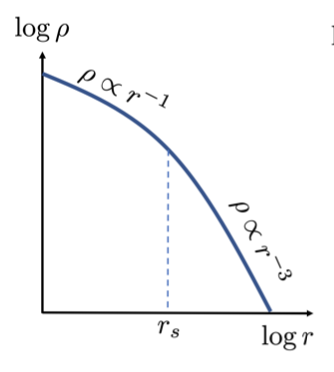
\includegraphics[width=1.0\linewidth]{NFW.png}
	\caption{NFW profile 示意图}
    \label{fig:NFW}
\end{figure}

NFW profile 存在一个问题 : Cusp-Core controversy. 
NFW profile 给出在靠近暗物质晕中心的区域, $\rho \propto r^{-1}$, 有一个高密度的“尖”,即 cusp.
但观测更倾向于 暗物质晕在中心区域密度不变, 即 “核”的结构 (core), $\rho \propto r^0$.
这对 冷暗物质理论提出了挑战。有人认为这说明 冷暗物质模型不对,他们提出了一些候选理论,比如温暗物质(warm dark matter),温暗物质是运动速度比冷暗物质快的一类粒子,这样它就会在暗物质晕形成时将中心密度较大区域的密度差异抹平。另一些人认为观测的是重子物质的分布,有可能重子物质分布和暗物质分布并不相同,重子物质在中心的分布是Core,而暗物质的分布是Cusp.
% ,用来推断


\section{暗物质晕的形成}

暗物质晕的形成也是 bottom-up scenario.
暗物质晕由小质量的晕通过并合逐渐增大的过程叫做 
Merger Tree. 如 \reffig{fig:MegerTree} 所示。

\begin{figure}[!hbtp]
	\centering 
	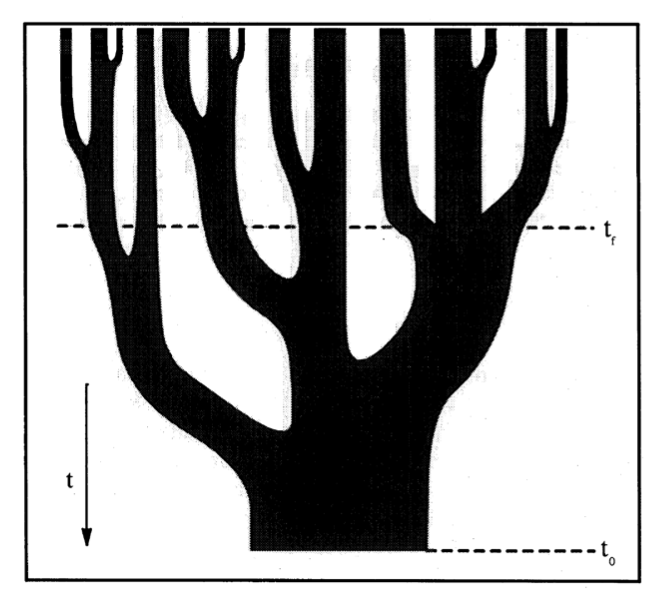
\includegraphics[width=1.0\linewidth]{MegerTree.png}
	\caption{Meger Tree 示意图}
    \label{fig:MegerTree}
\end{figure}

并合的过程也叫做 assembly history ,
assembly history 会影响 暗物质晕的性质,因此是目前重要的研究方向之一。

在暗物质晕的形成中,我们关心不同质量的暗物质晕分别会形成多少。
一个近似的方法是
随机行走 (Random Walk) of dark matter halo statistics.
物质密度的空间分布是随机的,当局部密度大于 临界密度 $\delta_\text{crit}$ 时,我们认为这里形成一个 暗物质晕。 如 \reffig{fig:RandomWalk} 所示,红色标出的区域是大小不同的暗物质晕。

\begin{figure}[!hbtp]
	\centering 
	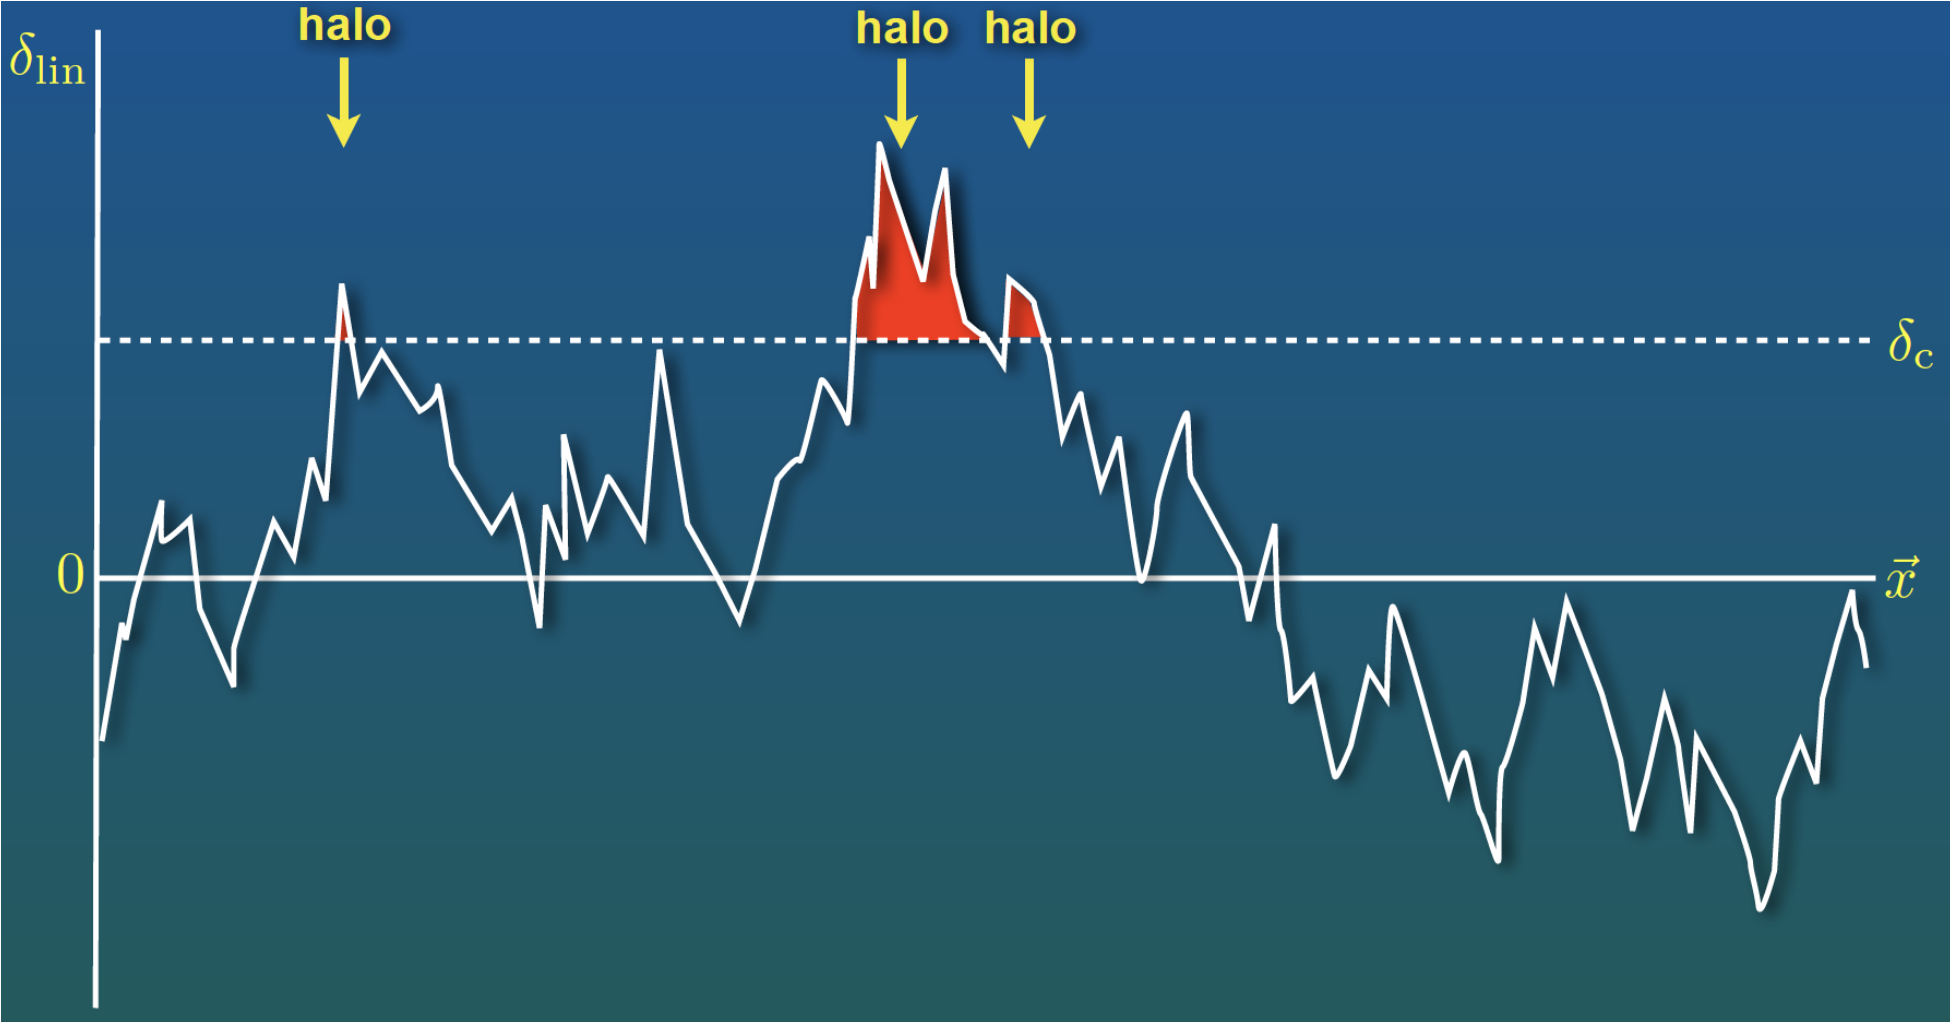
\includegraphics[width=1.0\linewidth]{Peaks_halo.png}
	\caption{Random Walk 示意图}
    \label{fig:RandomWalk}
\end{figure}

在 半径 $R$ 的范围内 对密度涨落做平滑: 
$\delta_M = \delta\left(\vec{x},R\right) $. 
这个平滑尺度对应 质量 $M=\bar{\rho} \times \frac{4}{3} \pi R^3$.

我们想计算 的 halo mass function 是 在一定质量范围内(大于$M$) halo 的数密度,
它 等于
在平滑尺度为 $M$ 时的  峰的 数密度
$n\left(>M\right) = n _{\rm{pk}} \left(\delta_M\right)$ .

Press-Schechter 模型
假设密度场是高斯分布
\begin{eqnarray}
    \mathcal{P}\left(\delta_{M}>\delta_{c}(t)\right) &=& F(>M, t) \\ 
    &=& \frac{1}{\sqrt{2 \pi} \sigma_{M}} \int_{\delta_{c}}^{\infty} \exp \left[-\frac{\delta_{M}^{2}}{2 \sigma_{M}^{2}}\right] d \delta_{M}=\frac{1}{2} \operatorname{erfc}\left[\frac{\delta_{c}}{2 \sigma_{M}}\right]
\end{eqnarray}
其中 $\operatorname{erfc}(x)=1-\operatorname{erf}(x)$, $\operatorname{erf}(x)=\frac{2}{\sqrt{\pi}} \int_{0}^{x} e^{-t^{2}} d t$ 是  error function.

\end{document}
